\subsection{sacabench batch}
\label{framework:cli:sacabench-batch}

{
    \begin{wrapfigure}[25]{r}[5mm]{.5\textwidth}
    \vspace{-1.5\baselineskip}
    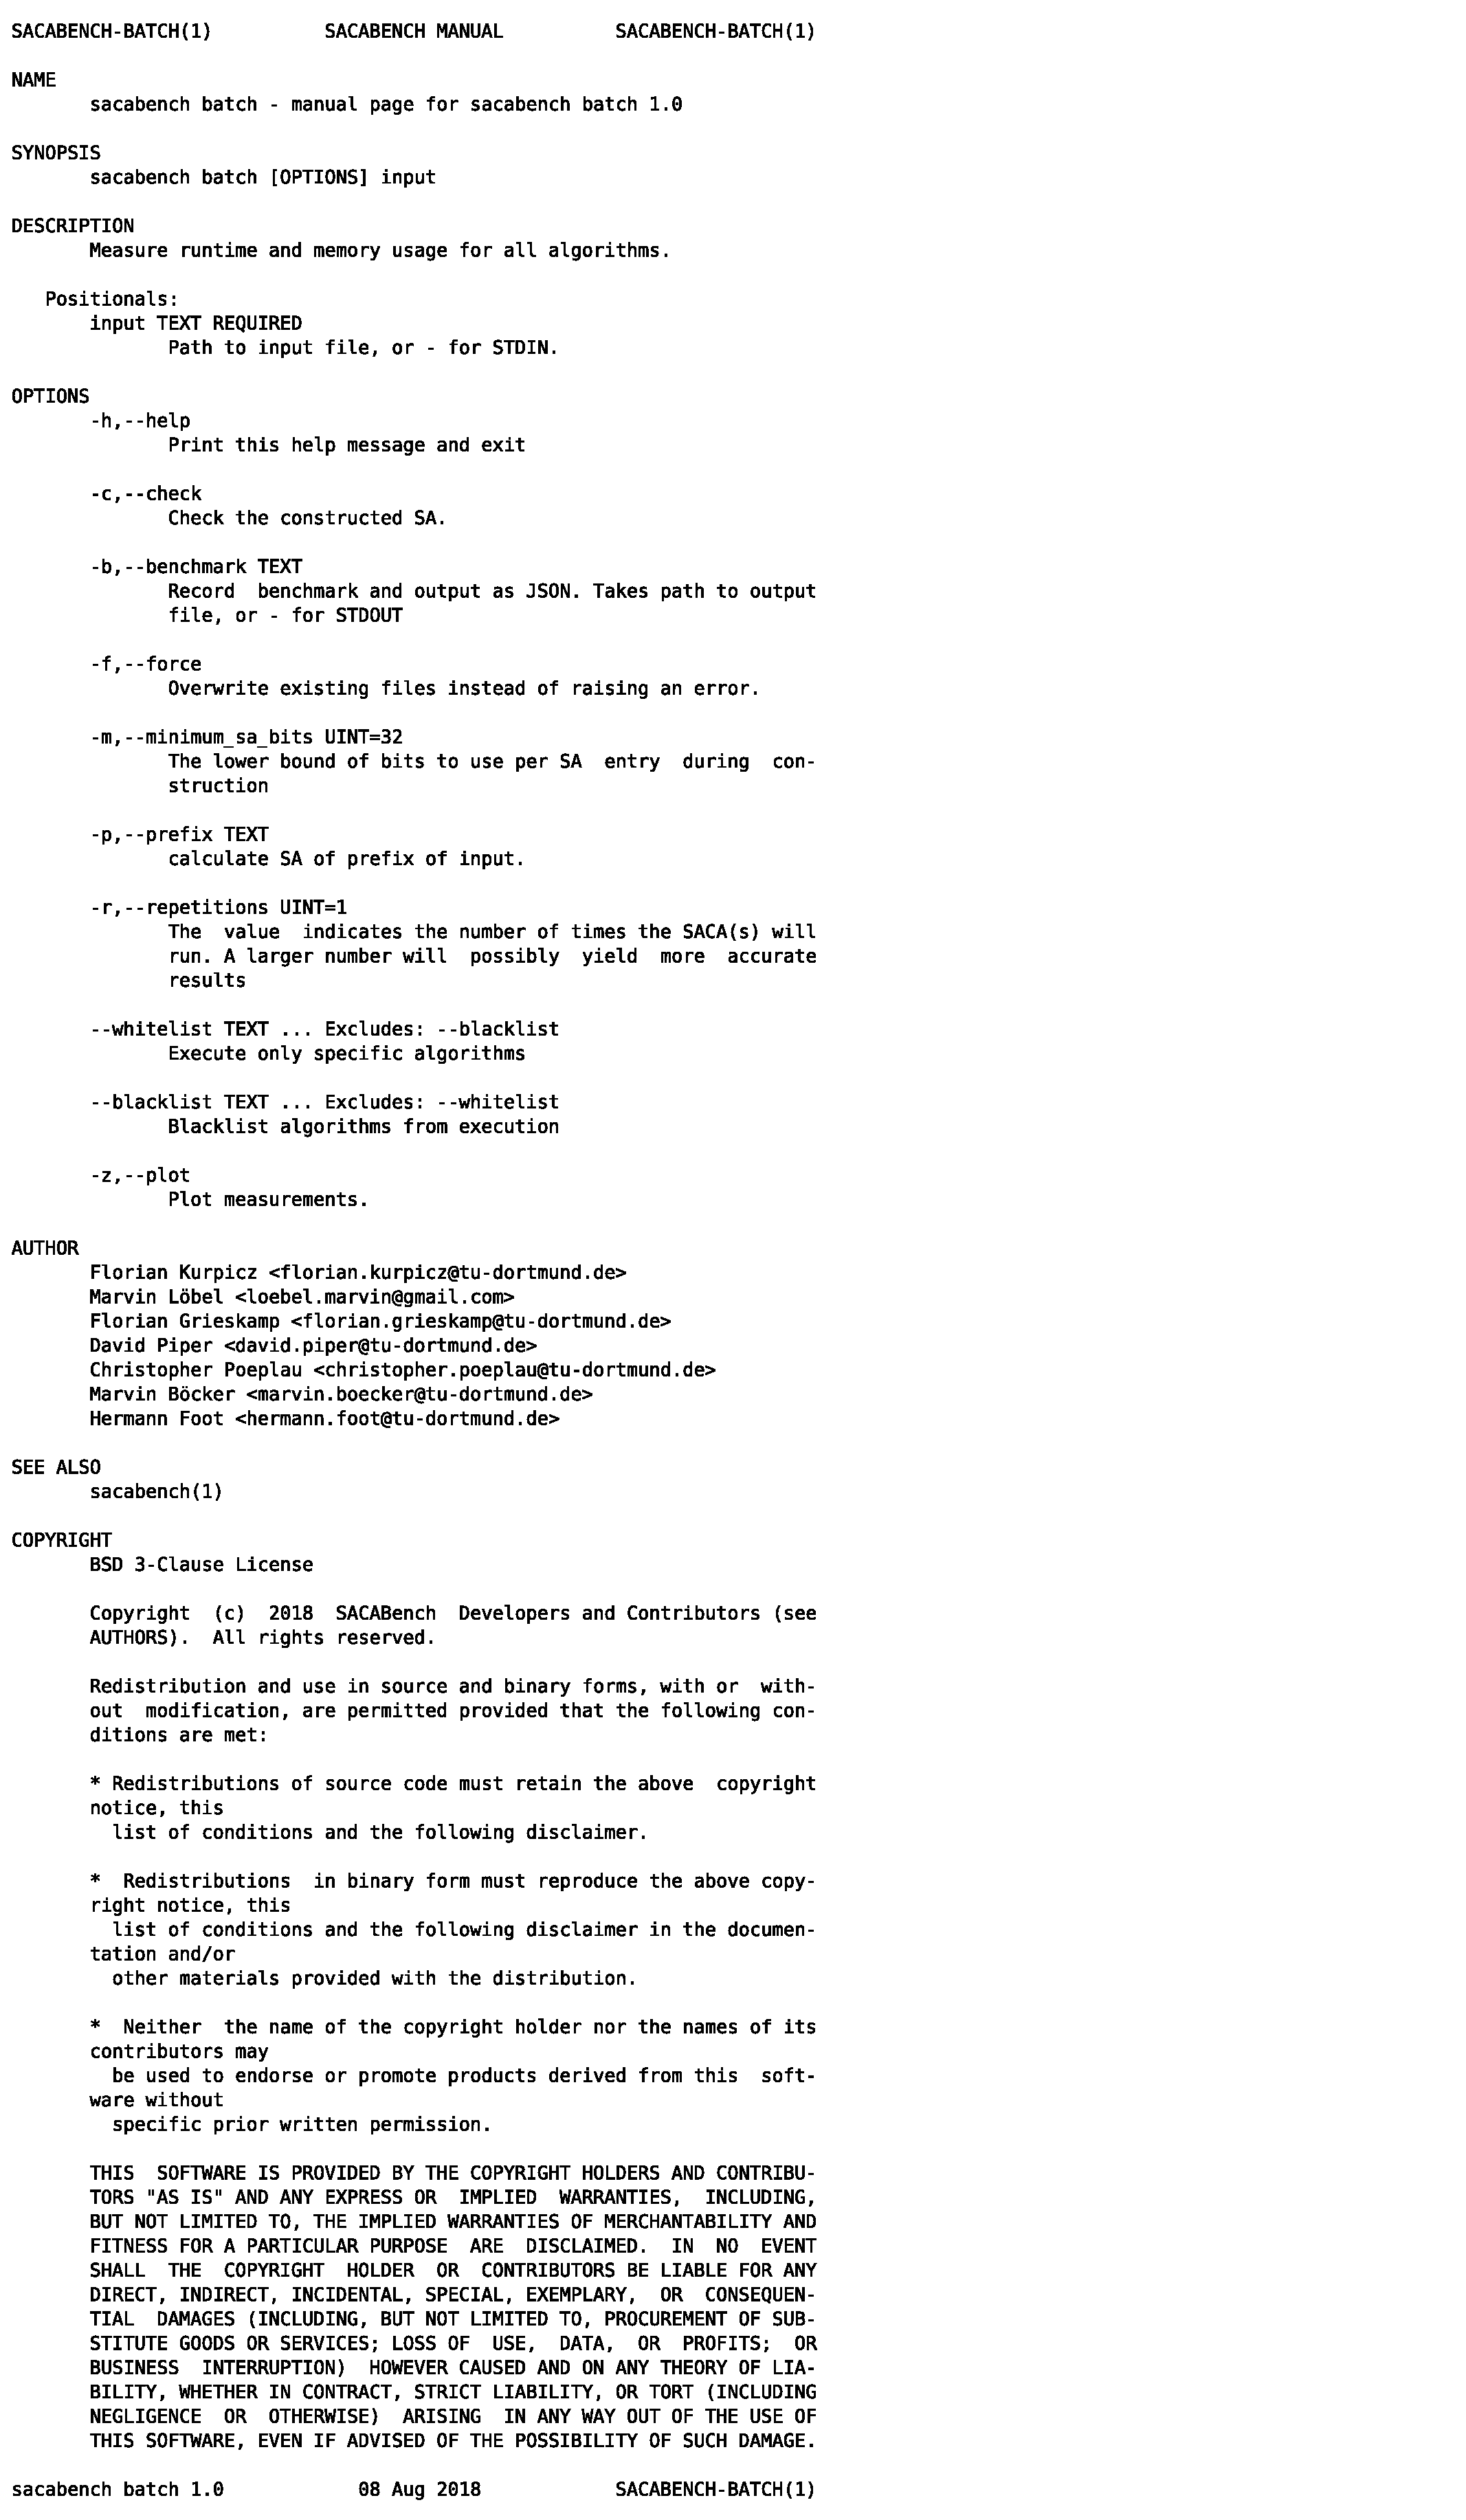
\includegraphics[page=1, viewport=0cm 32.8cm 20.5cm 62.0cm, clip, width=.5\textwidth]{{kapitel/3_framework/cli/sacabench-batch/sacabench-batch}.pdf}\\
    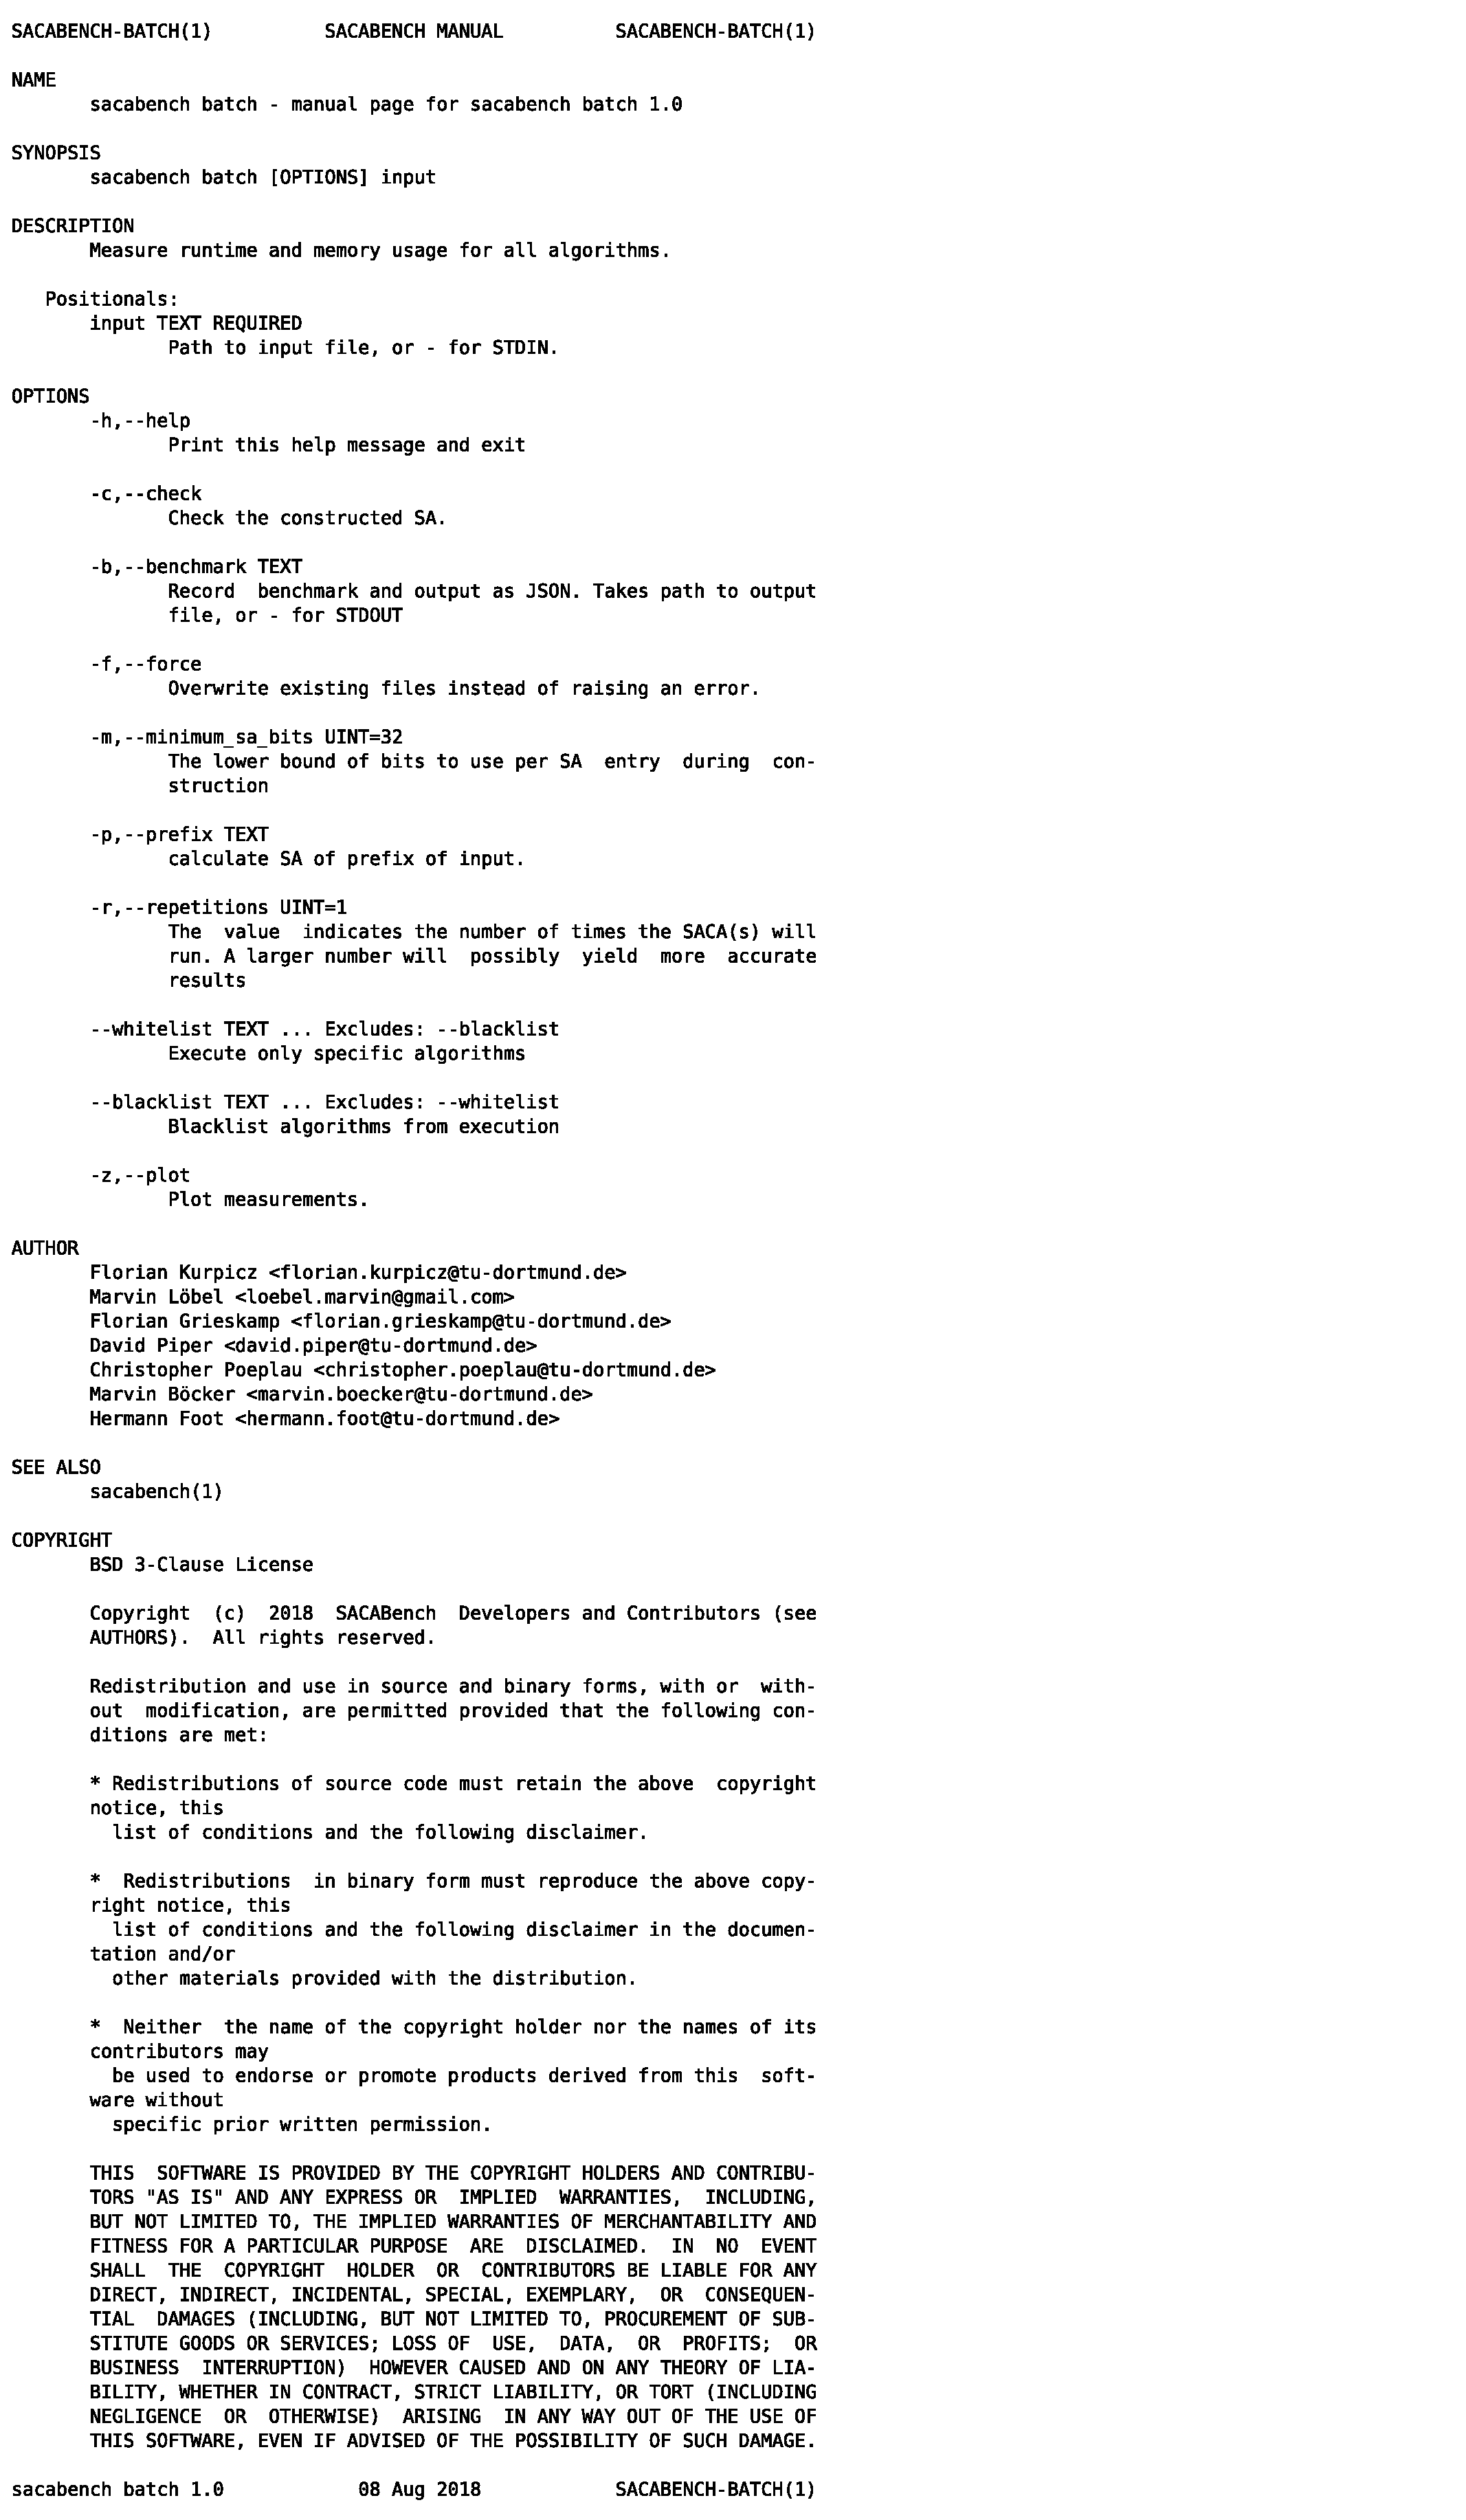
\includegraphics[page=1, viewport=0cm 25cm 20.5cm 26.3cm, clip, width=.5\textwidth]{{kapitel/3_framework/cli/sacabench-batch/sacabench-batch}.pdf}\\
    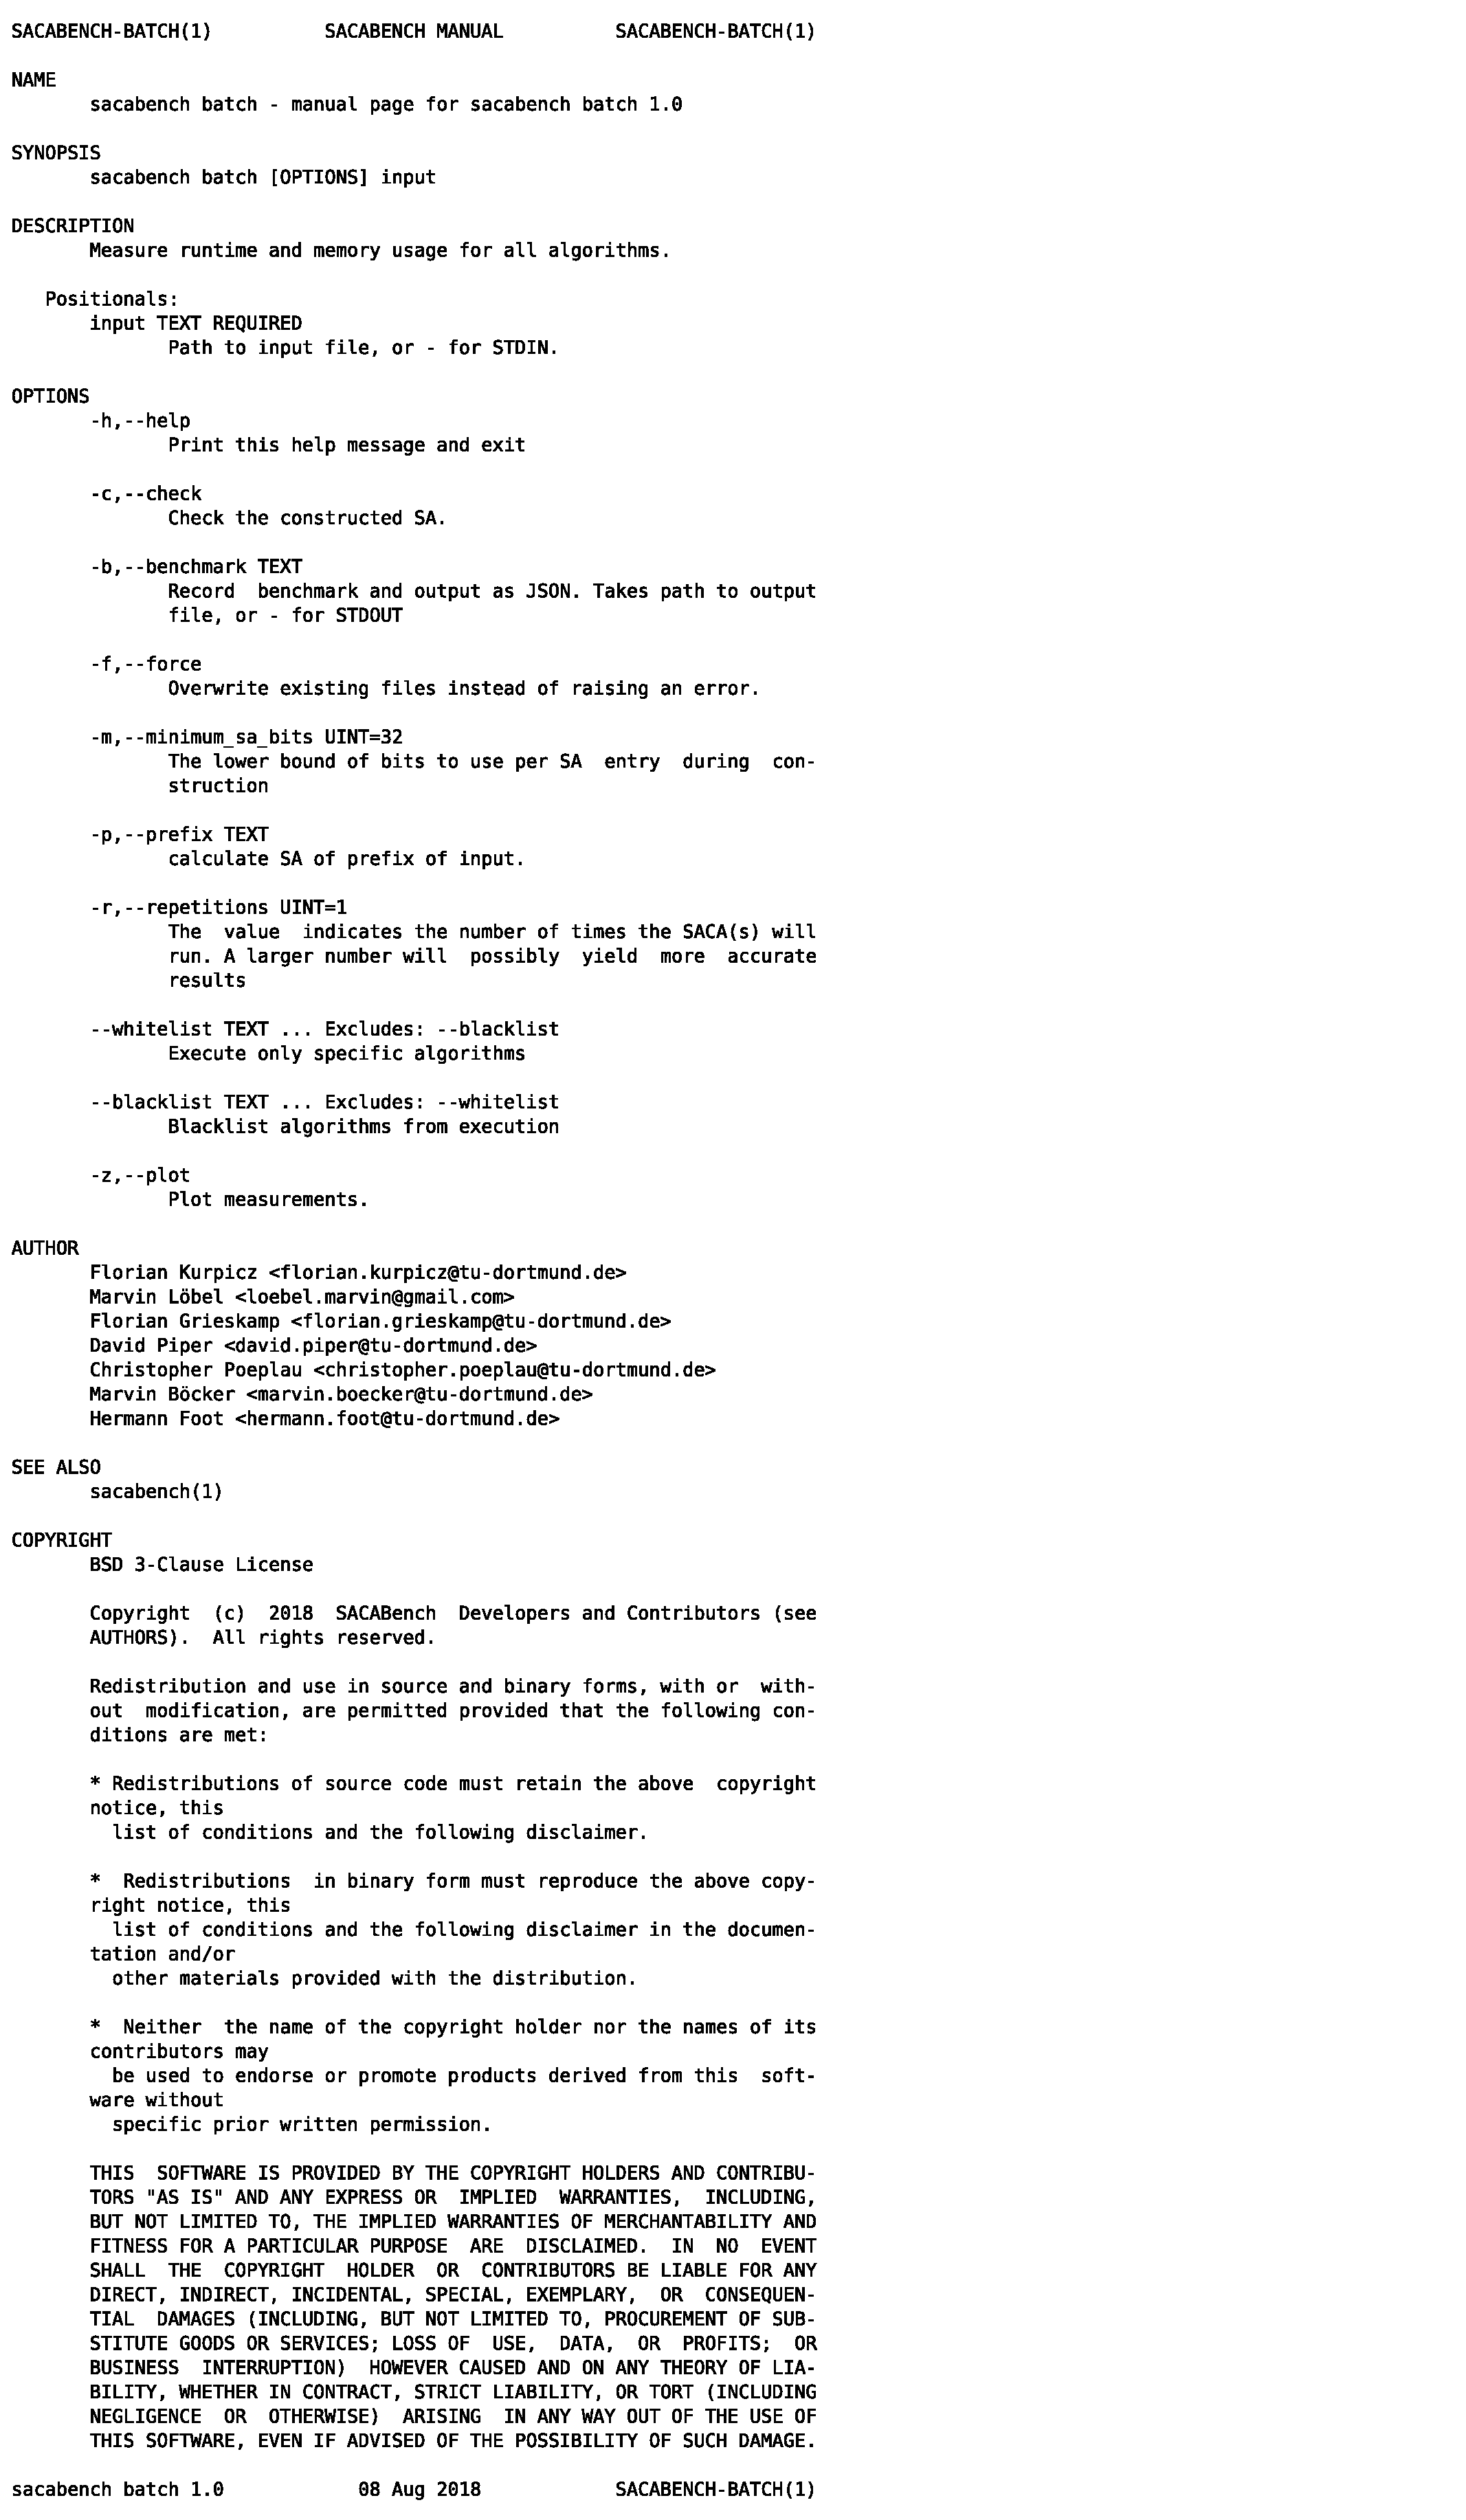
\includegraphics[page=1, viewport=0cm 0cm 20.5cm 1.5cm, clip, width=.5\textwidth]{{kapitel/3_framework/cli/sacabench-batch/sacabench-batch}.pdf}
    \caption{Gekürzte Ausgabe von \texttt{man sacabench batch}.}
    \label{manpage:sacabench-batch}
\end{wrapfigure}

Mit dem Befehl \texttt{sacabench batch} können mehrere Algorithmen auf der gleichen Eingabedatei ausgeführt werden. 
Die Funktionalität setzt hautpsächlich auf dem Interface von \termfont{sacabench construct} auf, weshalb ein Großteil der dort verwendbaren Optionen auch hier Anwendung findet. 
Zu beachten ist jedoch, dass die Ausgaben aller Algorithmen nach der Ausführung und einem optionalen Test auf Korrektheit verworfen werden. 
Alle das Ausgabeformat betreffenden Optionen von \termfont{sacabench construct} sind daher für \termfont{sacabench batch} ungültig.\par
Um nicht für jede Messung alle Algorithmen ausführen zu müssen, besteht die Option, wahlweise mit \termfont{-{}-blacklist} einzelne Algorithmen von der Ausführung auszuschließen oder mit \termfont{-{}-white\-list} nur explizit angegebene Algorithmen zu berechnen. 
Für beide Optionen entsprechen die Namen der anzugebenden Algorithmen denen aus \termfont{sacabench list} (\cref{framework:cli:sacabench-list}).
Benchmarks können wie genau wie zuvor mit \termfont{-{}-benchmark} unter Angabe eines Dateinamens angelegt werden. 
Die mit \termfont{-{}-plot} generierten Diagramme unterscheiden sich jedoch von den mit \termfont{sacabench construct} erstellten Diagrammen: 
Der Schwerpunkt liegt hier auf der Vergleichbarkeit der Algorithmen, weshalb in den Diagrammen gezielt die Laufzeit- und Speichermessungen aller ausgeführten Algorithmen miteinander verglichen werden. 
Eine ausführlichere Beschreibung der Diagramme sowie der zur Aufzeichnung der Benchmarks verwendeten Techniken ist im nächsten Abschnitt zu finden.\par
}
